\documentclass{beamer}

\usetheme{Warsaw}
\usecolortheme{seahorse}

\usepackage{amsfonts}

\usepackage[french]{babel}
\usepackage[utf8]{inputenc}
\usepackage[T1]{fontenc}


\begin{document}

\title{Bandits et Plannification}

\author{Arpad Rimmel}
\institute{SUPELEC}

\AtBeginSection[]
{
    \begin{frame}
        \frametitle{Table des matières}
        \tableofcontents[currentsection]
    \end{frame}
}


\begin{frame}
    \titlepage
\end{frame}

\begin{frame}
    \frametitle{Table des matières}
    \tableofcontents[]
\end{frame}


\section*{Introduction}

\begin{frame}
    \frametitle{Exemple de problème}
    \begin{center}
        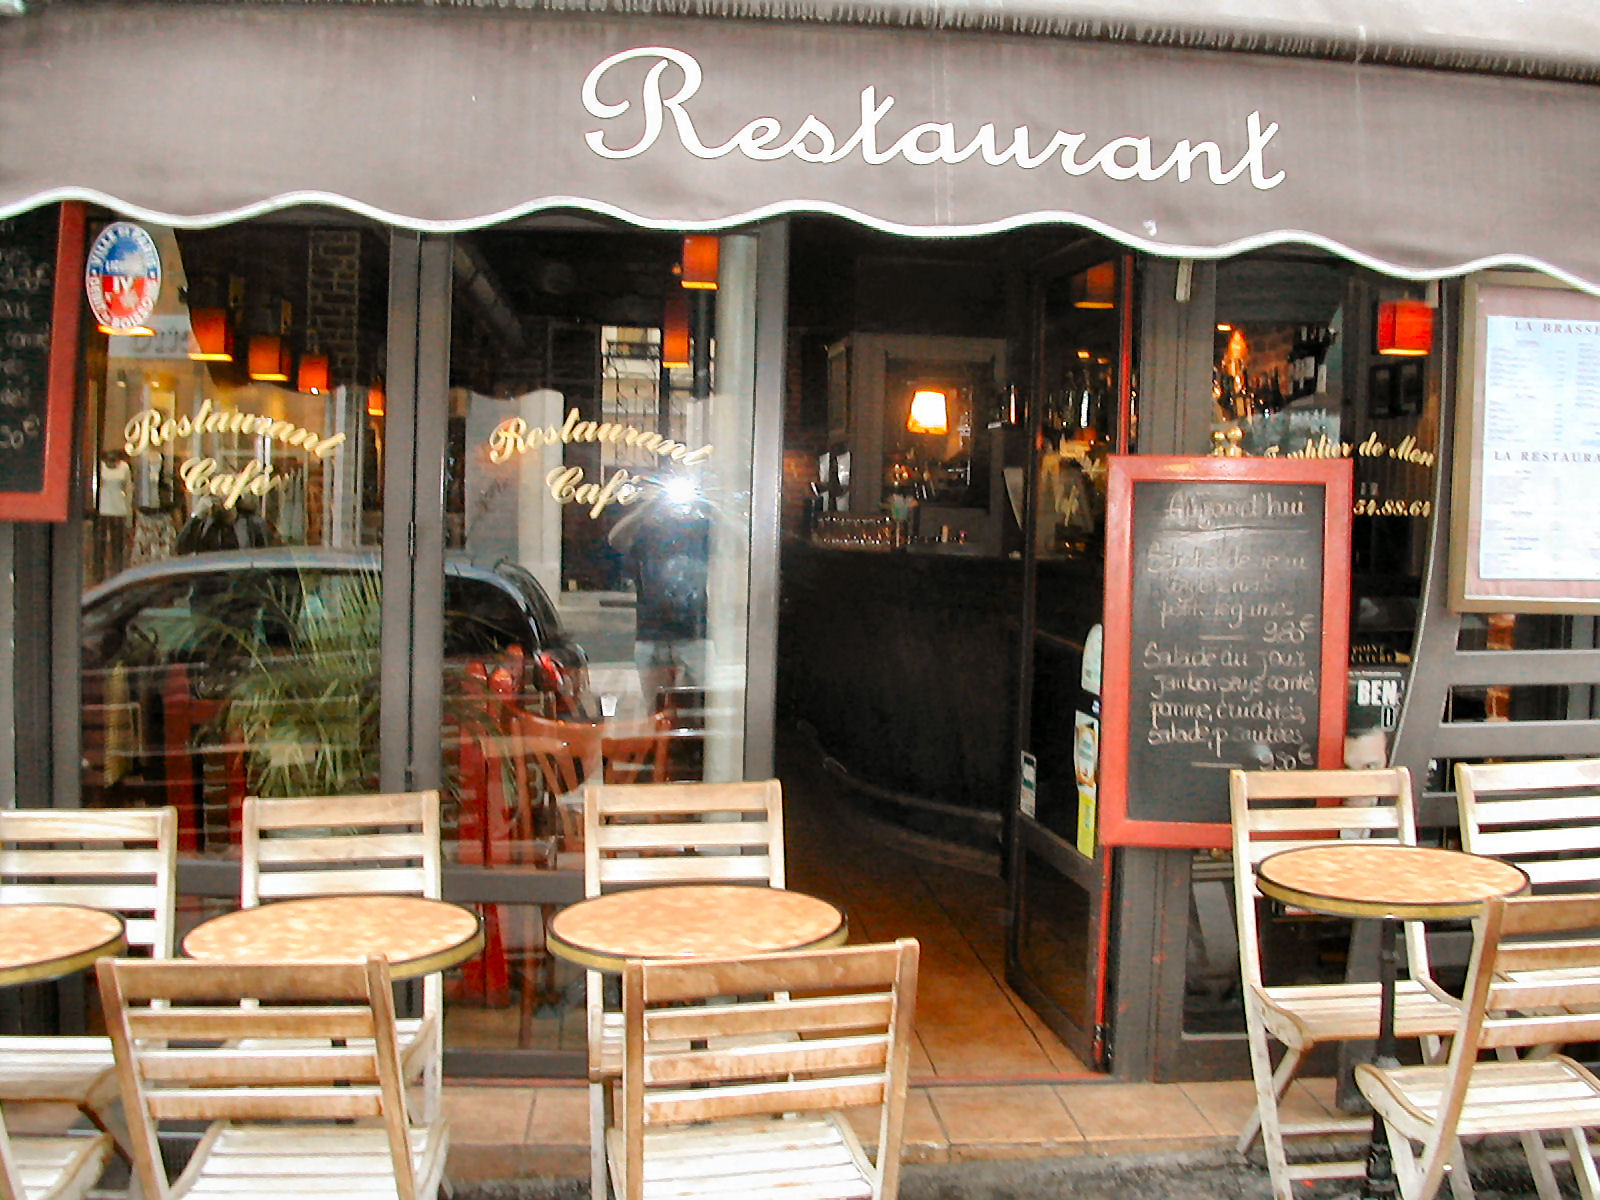
\includegraphics[scale=0.05]{restau.jpg}
    \end{center}
    Problème:
    \begin{itemize}
        \item Vous allez au restaurant tout les 3-4 jours  pendants 1 an (100 fois).
        \item Il y a 10 restaurants dans le quartier.
        \item Vous voulez déterminer quel est LE meilleur restaurant du quartier.
    \end{itemize}
\end{frame}

\begin{frame}
    \frametitle{Exemple de problème}
    \begin{center}
        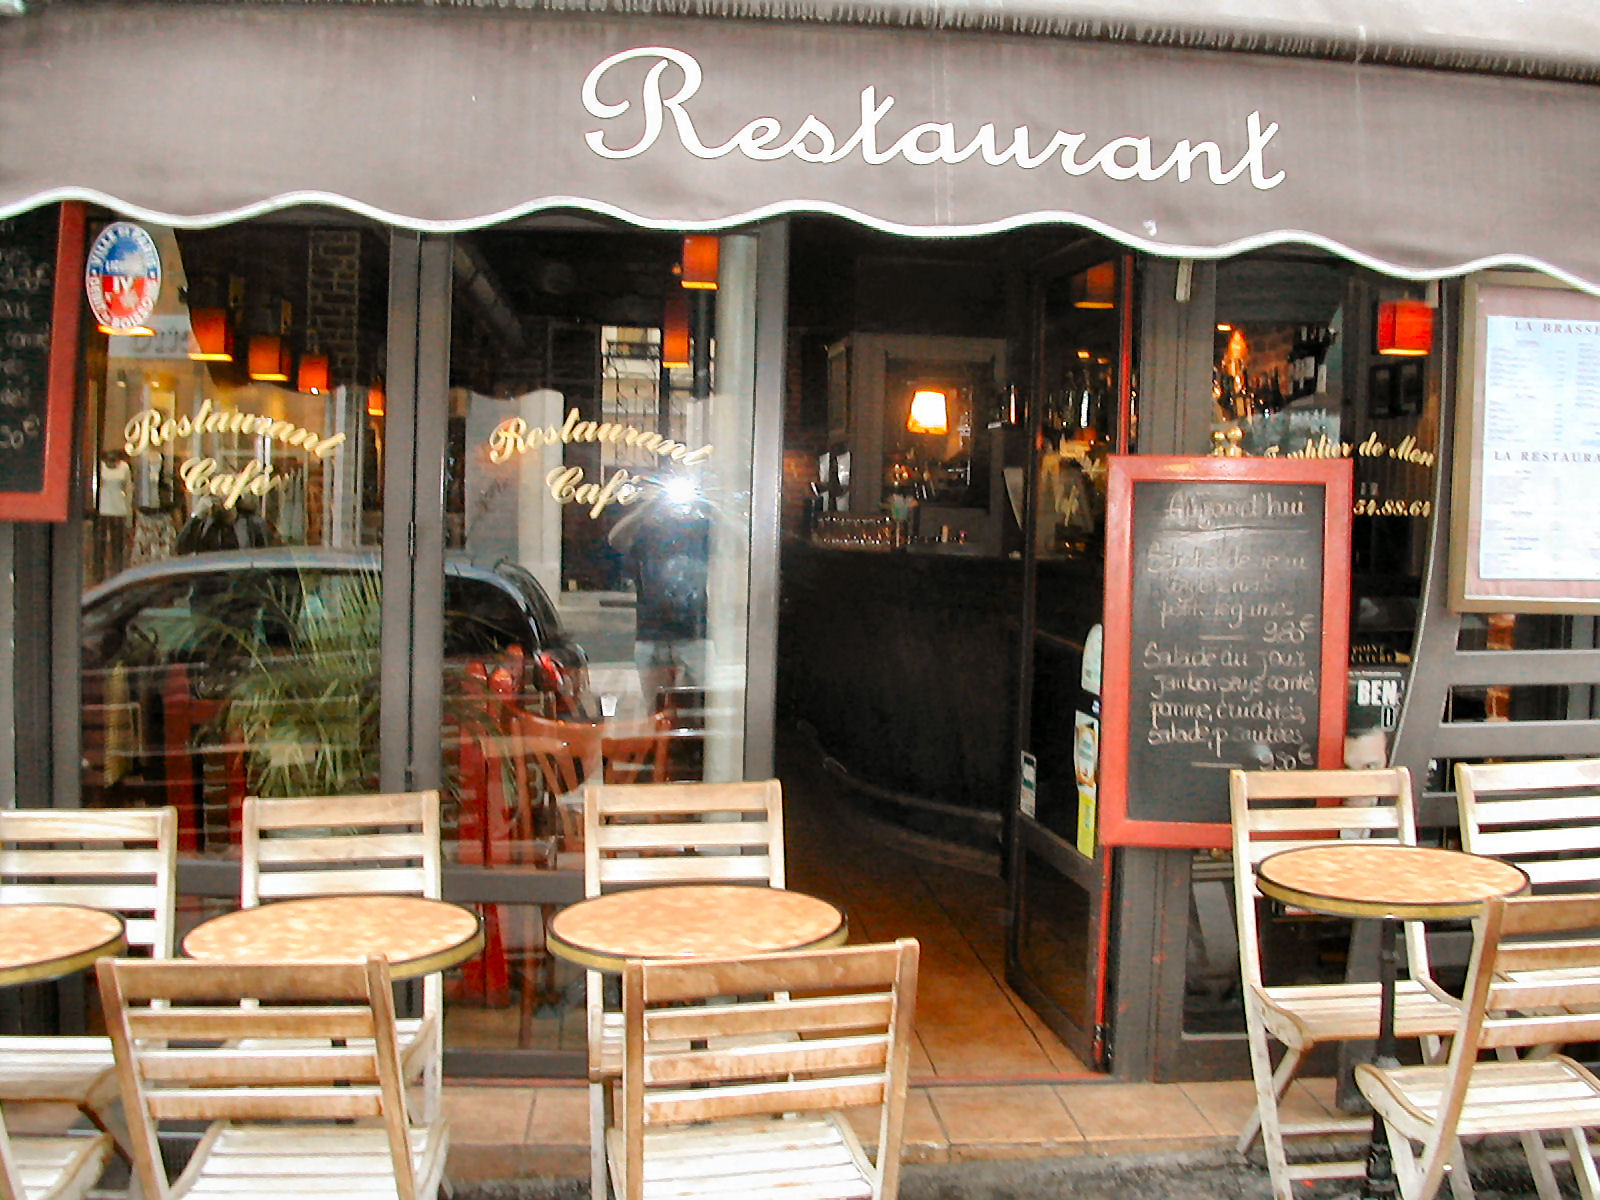
\includegraphics[scale=0.05]{restau.jpg}
    \end{center}
    Solutions?:
    \begin{itemize}
        \item Tester chaque restaurant 10 fois?
        \item Tester chaque restaurant 4 fois puis les 3 meilleurs 20 fois?
        \item Tester chaque restaurant 1 fois puis les 3 meilleurs 30 fois?
    \end{itemize}
\end{frame}

\begin{frame}
    \frametitle{Intuition}
    la plupart des algorithmes seront basés sur un compromis entre:
    \begin{itemize}
        \item sélectionner le restaurant qui a obtenu la meilleure note  :
        \item essayer un restaurant peu essayé jusqu'ici:
    \end{itemize}

    \begin{center}
        {\color{red}EXPLOITATION} vs {\color{green}EXPLORATION}
    \end{center}

\end{frame}

\begin{frame}
    \frametitle{Autres Exemples de problèmes}
    \begin{center}
        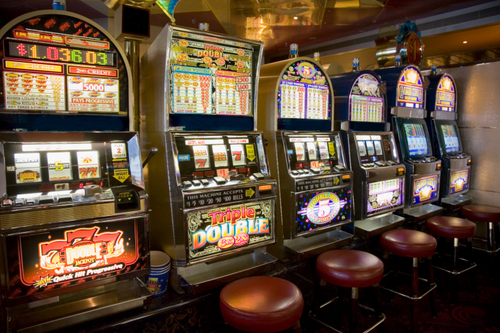
\includegraphics[scale=0.8]{bandit_casino.jpg}
    \end{center}
    \begin{itemize}
        \item Les bandits manchots: trouver la machine qui rapporte le plus.
        \item Essais cliniques: trouver le traitement qui fonctionne le mieux.
        \item Sélection d'un serveur dans un réseau: trouver le serveur avec le temps de réponse le plus faible.
        \item Publicité ciblée: trouver le type de pub qui intéressera le plus un utilisateur.
        \item ...
    \end{itemize}
\end{frame}


\begin{frame}
    \frametitle{Définition formelle}
    \begin{center}
        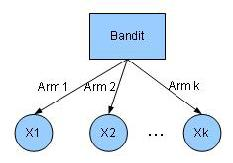
\includegraphics[scale=0.5]{bandit.jpg}
    \end{center}
    \begin{itemize}
        \item un ensemble de bras $A=\{1,...,K\}$.
        \item chaque bras est associé à une distribution de probabilité $X_k$ d'espérance $\mu_k$.
        \item l'algorithme choisit un bras $a$ à chaque pas de temps.
        \item le bandit retourne une récompense $r$ : une réalisation de $X_a$.
        \item les tirages successifs sur un même bras sont indépendant et identiquement distribués.
    \end{itemize}
\end{frame}



\begin{frame}
    \frametitle{Notations supplémentaires}
    \begin{itemize}
        \item $T_i(n)$: le nombre de fois que le bras $i$ a été sélectionné au pas de temps $n$.
        \item $\mu^* = \max_{1 \le i \le K}\mu_i$
        \item $\Delta_i = \mu^* - \mu_i$ 
        \item $\Delta = \min_{i:\Delta_i > 0}\Delta_i$
    \end{itemize}


\end{frame}

\section{Bandit classique}

\begin{frame}
    \frametitle{Objectif}

    Le but est d'optimiser le regret $R_n$ défini comme suit:

    $$R_n=\mu^*n - \mathbb{E} \sum_{j=1}^{K}  T_j(n) \mu_j$$
    $$R_n=\sum_{j=1}^{K} \Delta_j \mathbb{E} [T_j(n)]$$

\end{frame}



\begin{frame}
    \frametitle{Borne inférieure}


    Pour toute stratégie d'allocation et pour tout bras non optimal:
    $$\mathbb{E} [T_j(n)] \ge \frac{\log n}{D(p_j || p^*)}$$

    $$\mbox{où }D(p_j || p^*) = \int p_j \log \frac{p_j}{p^*}$$
    On en déduit que le meilleur regret atteignable est en ${\color{red} \log(n)}$.

    \hfill [Lai and Robbins, 1985]

\end{frame}


\begin{frame}
    \frametitle{Epsilon greedy}
    Principe de l'algorithme:

    A chaque pas de temps $t$
    \begin{itemize}
        \item avec probabilité {\color{red}$1 - \epsilon_t$}, on sélectionne le bras avec la moyenne empirique la plus élevée.
        \item avec probabilité {\color{green}$\epsilon_t$}, on sélectionne un bras au hasard.
    \end{itemize}
    $\epsilon_t$ décroit avec le temps.

    \hfill [Auer and all, 2002]
\end{frame}

\begin{frame}
    \frametitle{Epsilon greedy}
    Propriétés théorique de l'algorithme avec {\color{blue} $\epsilon_t = \min(\frac{6K}{\Delta^2t},1)$}.

    Quand $t \ge \frac{6K}{\Delta^2}$, la probabilité de choisir un bras sous optimal est bornée par $\frac{C}{\Delta^2t}$ où $C$ est une constante strictement positive.

    En conséquence, $\mathbb{E} [T_j(n)] \le \frac{C}{\Delta^2}\log(n)$ et donc 

    $$ R_n \le \sum_{i:\Delta_i>0} \frac{C\Delta_i}{\Delta^2}{\color{red} \log(n)} $$

\end{frame}

\begin{frame}
    \frametitle{Epsilon greedy}
    Défauts de l'algorithme:
    \begin{itemize}
        \item exploration naïve des bras
        \item nécessite de connaitre $\Delta$
    \end{itemize}
\end{frame}



\begin{frame}
    \frametitle{UCB}
    Principe de l'algorithme:
    \begin{itemize}
        \item A partir des informations disponibles au temps $t$, on calcule la borne de confiance supérieur (UCB) correspondant à chaque bras.
        \item On choisit le bras qui a la valeur UCB la plus grande.
    \end{itemize}
    \hfill [Auer and all, 2002]
\end{frame}

\begin{frame}
    \frametitle{UCB}
    Calcul de la valeur UCB pour le bras $i$ au pas de temps $t$:
    $$ {\color{red} \hat{\mu}_{i,t-1}} + {\color{green} \sqrt{\frac{3\log(t)}{2T_i(t-1)}}} $$
    où $\hat{\mu}_{i,t-1} $ correspond à la moyenne empirique du bras $i$.
    
\end{frame}

\begin{frame}
    \frametitle{UCB}
    Borne sur le regret:
    $$ R_n \le 6*\sum_{i \ne i^*}\frac{\color{red}\log(n)}{\Delta_i} + K(\frac{\pi^2}{3}+1) $$
    
\end{frame}



\begin{frame}
    \frametitle{UCB en pratique}
    \begin{itemize}
        \item Ajout d'un paramètre $p$ de contrôle de l'exploration:
            $$ \hat{\mu}_{i,t-1} + {\color{blue}p} \sqrt{\frac{\log(t)}{T_i(t-1)}} $$
        \item Ajout de connaissances a priori $C_i(t)$:
            $$ \hat{\mu}_{i,t-1} + p \sqrt{\frac{\log(t)}{T_i(t-1)}} + {\color{blue} C_i(t)} $$
    \end{itemize}
    
\end{frame}

\section{Variantes du bandit}

\begin{frame}
    \frametitle{Nombreuses Variantes}
    \begin{itemize}
        \item différents environnements: {\color{blue}stochastique}, adversarial, non-stationnaire, ...
        \item différents buts: {\color{blue}regret cumulé}, regret simple, trouver la meilleur valeur, ...
        \item nombre de bras {\color{blue}fini} ou infini
        \item ajout de règles: paiement à chaque essai, paiement pour changer de bras, nombre de bras qui varie, ...
        \item forme de la distribution connue
    \end{itemize}
\end{frame}


\begin{frame}
    \frametitle{nombre de bras infini}
    Problème quand le nombre de bras est infini ou grand par rapport aux nombres d'essais:

    \begin{itemize}
        \item les algorithmes classiques commencent par essayer une fois chaque bras.
    \end{itemize}

    Exemples d'application:
    \begin{itemize}
        \item recherche du meilleur restaurant à Paris 
        \item recherche d'emplacement de ressources précieuses (or, pétrole, ...)
    \end{itemize}

\end{frame}

\begin{frame}
    \frametitle{progressive widening}

    Utiliser uniquement $K(t)$ bras au temps $t$
    $$ K(t) = t^\alpha \mbox{ avec } \alpha \in [0.25,0.5]$$

    Les bras peuvent être choisis selon une heuristique ou au hasard.

    \hfill [Coulom, 2007]

    \hfill [Chaslot, 2007]

\end{frame}

\begin{frame}
    \frametitle{Maximiser la meilleure valeur}

    Différences avec le bandit classique:
    \begin{itemize}
        \item Seul le meilleur résultat est conservé.
        \item Il ne faut plus trouver le bras avec la meilleure espérance, la variance doit aussi être prise en compte.
        \item La notion de regret ne s'applique plus.
    \end{itemize}

    Exemples d'applications: 
    \begin{itemize}
        \item recherche de meilleur trajet
    \end{itemize}

\end{frame}

\begin{frame}
    \frametitle{Threshold Ascent}

    Principe:
    \begin{itemize}
        \item Calcul d'une valeur pour chaque bras et à chaque pas de temps
        \item Sélectionner le bras avec la plus grande valeur
        \item La valeur est basée sur le compromis exploitation/exploration
        \item l'exploitation est basée sur le nombre de fois que le bras a obtenu une réponse faisant parti des $s$ meilleures
    \end{itemize}

    \hfill [Streeter and Smith, 2006]

\end{frame}

\begin{frame}
    \frametitle{environnement non stationnaire}
    Différences avec le bandit classique:
    \begin{itemize}
        \item Les variables aléatoires varient au court du temps
        \item vrai dans beaucoup de cas en pratique
        \item Nécessité d'imposer des contraintes sur ces variations
    \end{itemize}

    Exemples d'applications: 
    \begin{itemize}
        \item recherche de restaurant (changement de chef)
        \item publicité ciblée (les préférences des utilisateurs changent)
        \item ...
    \end{itemize}


\end{frame}

\begin{frame}
    \frametitle{environnement non stationnaire}

    Cas ou les changements sont "brusques":
    \begin{itemize}
        \item entre 2 pas de temps, un variable aléatoire peut être modifiée
        \item la nouvelle variable aléatoire est alors fixe pendant un nombre de pas de temps aléatoire
    \end{itemize}

    Solution:
    \begin{itemize}
        \item Discounted UCB:
            le terme d'exploitation est calculé en mettant un poids plus fort aux derniers résultats.
        \item Sliding-Window UCB:
            le terme d'exploitation est calculé sur une fenêtre de temps glissante.
    \end{itemize}

    \hfill [Garivier and Moulines, 2008]

\end{frame}

\section{Bandits pour la planification}


\begin{frame}
    \frametitle{définition du problème}
    Le but est de prendre une décision dans un environnement:
    \begin{itemize}
        \item observable
        \item discret
        \item à horizon fini
        \item avec un espace d'état trop grand pour être exploré en entier
    \end{itemize}

    \begin{center}
        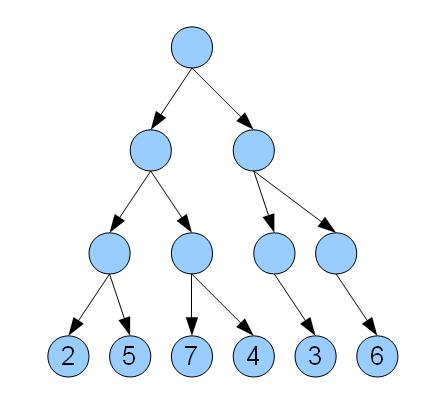
\includegraphics[scale=0.3]{arbre.jpg}
    \end{center}

\end{frame}

\begin{frame}
    \frametitle{Exemples d'applications}
    \begin{itemize}
        \item gestion de production
        \item apprentissage actif
        \item multiplication rapide de matrices
        \item jeu de go
    \end{itemize}

    \begin{center}
        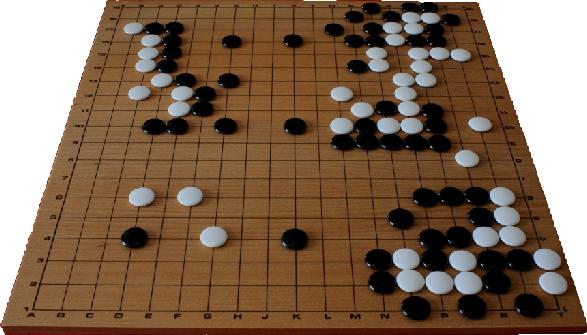
\includegraphics[scale=0.2]{go.jpg}
    \end{center}

\end{frame}


\begin{frame}
    \frametitle{présentation de l'algorithme}
    Principe:
    \begin{itemize}
        \item construction itérative d'un sous arbre en mémoire
        \item sous arbre déséquilibré vers les parties intéressantes de l'arbre
    \end{itemize}

    \begin{center}
        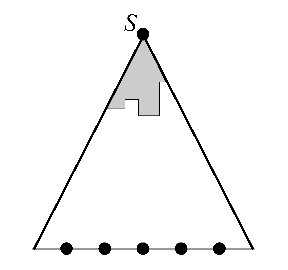
\includegraphics[scale=0.4]{arbre_desequilibre.jpg}
    \end{center}


\end{frame}

\begin{frame}
    \frametitle{Algorithme}

    Pour cela, on répète ces 3 étapes jusqu'au critère d'arrêt:
    \begin{itemize}
        \item Descente

            On parcourt le sous arbre en mémoire jusqu'à atteindre un nœud à la frontière de l'arbre.

        \item Évaluation

            On évalue ce nœud grâce à une fonction d'évaluation non déterministe (Monte Carlo ou autre).
        \item Mise à jour

            On ajoute le nœud à l'arbre et on met à jour les informations de l'arbre.
    \end{itemize}


\end{frame}

\begin{frame}
    \frametitle{Algorithme}
    \begin{center}
        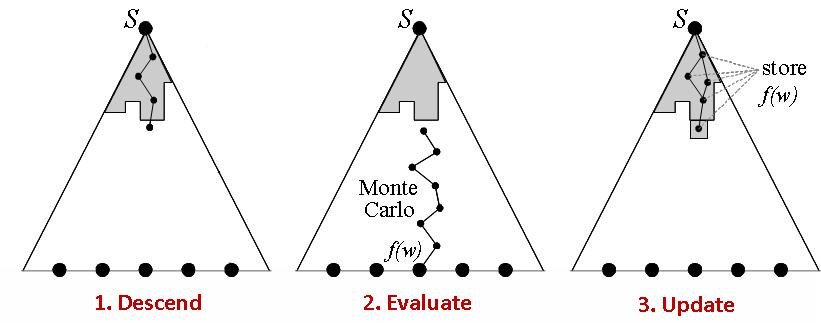
\includegraphics[scale=0.5]{3steps.jpg}
    \end{center}


\end{frame}

\begin{frame}
    \frametitle{Descente dans l'arbre}
    La descente dans l'arbre se fait en considérant que chaque choix d'une branche est un problème de bandit.

    \begin{center}
        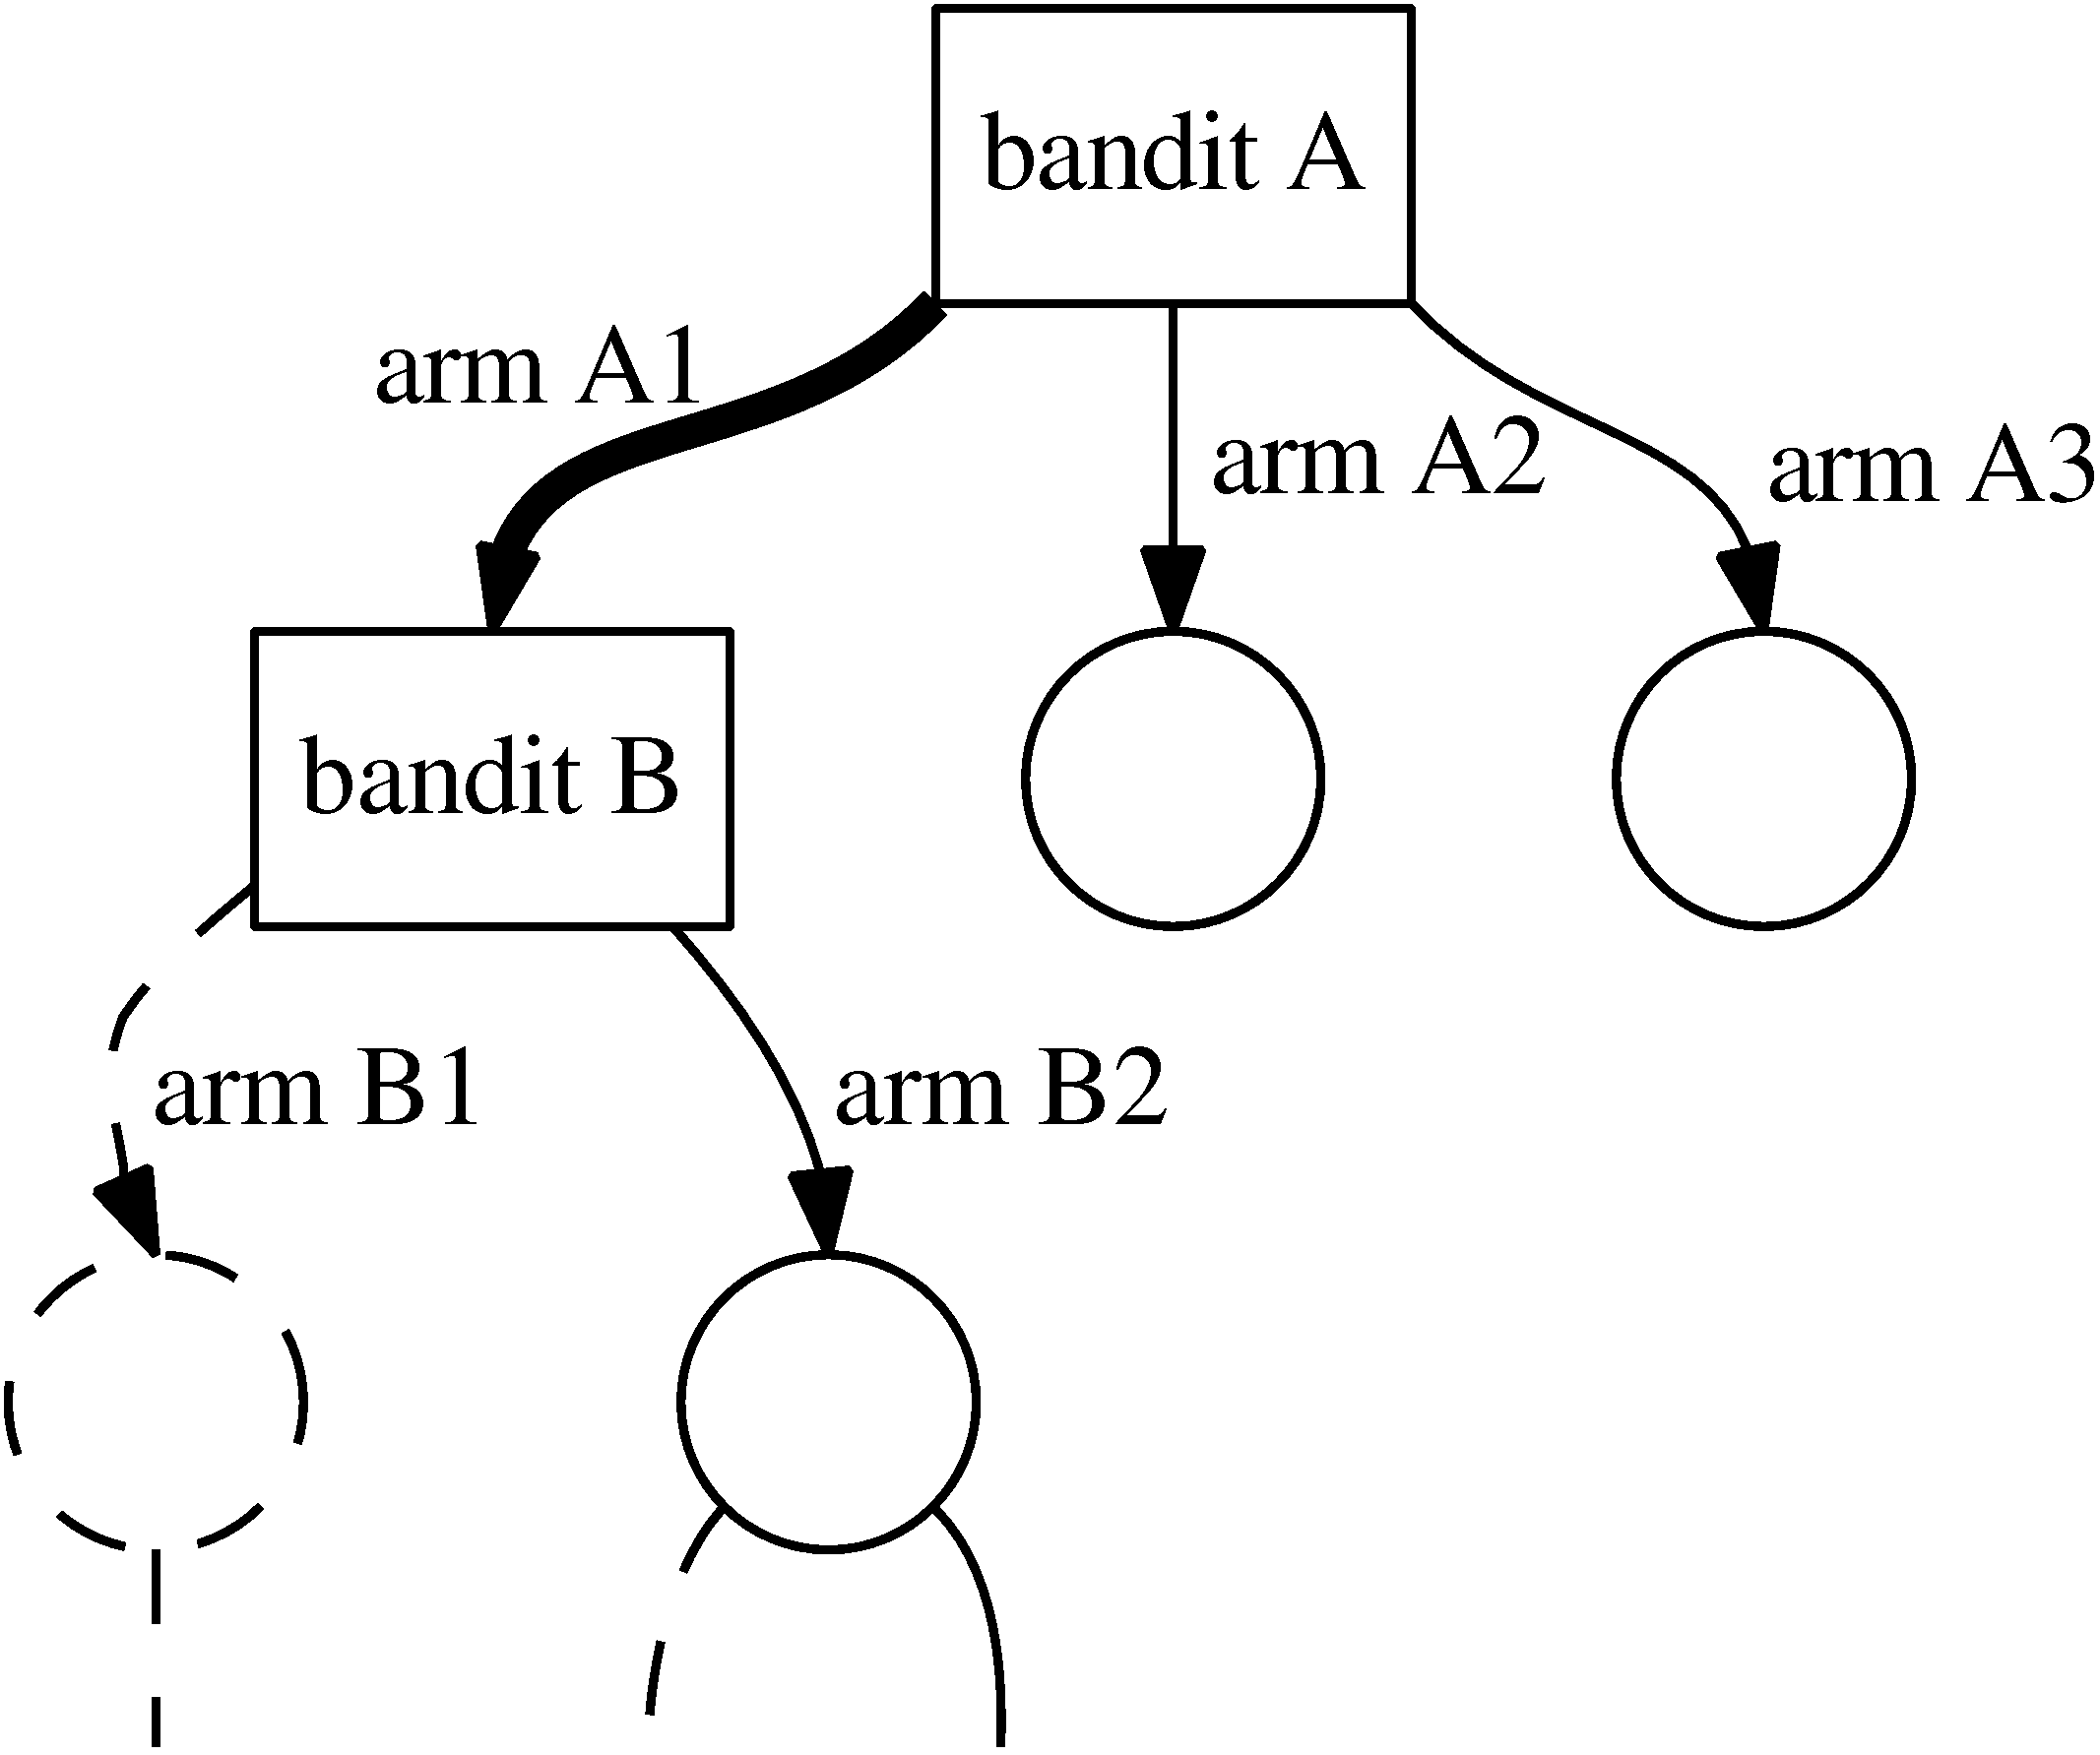
\includegraphics[scale=0.5]{bandit_cascade.png}
    \end{center}


\end{frame}

\begin{frame}
    \frametitle{En pratique}

    Le bandit qu'il faudrait considérer est différent du bandit classique:
    \begin{itemize}
        \item proche des feuilles du sous arbre, le nombre de tentative est faible face au nombre de possibilités
        \item regret simple
        \item les variables aléatoires évolues en fonction du temps (pas de manière brusque)
        \item les tirages ne sont pas iid
    \end{itemize}


\end{frame}

\begin{frame}
    \frametitle{Exemples}

    Exemples d'applications:
    \begin{itemize}
        \item Jeux de plateau à 2 joueurs: Go, Havannah, ...

            UCB modifié + Progressive Widening + connaissances
        \item Jeux à un joueur: multiplication de matrices

            Threshold Ascent  
    \end{itemize}

\end{frame}


\begin{frame}
    \frametitle{Remarques}
    \begin{itemize}
        \item fonction d'évaluation a beaucoup d'impact
        \item ordre pour explorer les bras a  beaucoup d'impact
        \item garantie de convergence à l'infini (car arbre exploré en entier)
        \item pas de garantie sur la vitesse de convergence

    \end{itemize}
    Peu se comporter moins bien qu'une recherche uniforme sur certains problèmes

    \hfill [Coquelin and Munos, 2007]

\end{frame}




\section*{Conclusion}

\begin{frame}
    \frametitle{conclusion}
    \begin{itemize}
        \item Le problème de bandit classique a beaucoup été étudié et de nombreux algorithmes ont été proposés qui possèdent de bonnes performances en théorie et en pratique.
        \item En fonction de l'application, une variante du bandit doit être utilisée. 
        \item Beaucoup de variantes du bandit n'ont pas ou peu été étudiées.
        \item L'utilisation de bandits pour explorer des arbres donne de bons résultats en pratique mais a peu été étudié de manière théorique.
    \end{itemize}
\end{frame}

\section*{Annexe}

\begin{frame}
    \frametitle{preuve de UCB}
    Rappel:
    $$R_n=\sum_{j=1}^{K} \Delta_j \mathbb{E} [T_j(n)]$$

    Principe:
    \begin{itemize}
        \item Borner $\mathbb{E} [T_j(n)]$ pour $j \ne j^*$
    \end{itemize}

    Moyen:
    \begin{itemize}
        \item Borne de Chernoff-Hoeffding
    \end{itemize}


\end{frame}

\begin{frame}
    \frametitle{Borne de Chernoff-Hoeffding}
    \begin{itemize}
        \item Soit $X_1,...,X_n$ des variables aléatoires dans $[0,1]$ tel que $\mathbb{E}[X_t|X_1,...,X_{t-1}]=\mu$
        \item Soit $S_n = X_1 + ... + X_n$
        \item alors pour tout $a\ge0$
            $$\mathbb{P}\{1/n*S_n \ge \mu + a\} \le e^{-2na^2} $$
        \item remarque: cette borne permet de relier la moyenne empirique d'une variable aléatoire avec sa moyenne théorique.
    \end{itemize}
    
\end{frame}

\begin{frame}
    \frametitle{preuve UCB}
    on en déduit pour tout $s$, tel que $1<s<t$:
    $$\mathbb{P}\{ \hat{\mu}_{k,s} + \sqrt{\frac{3\log(t)}{2s}} \le \mu_k\} \le e^{-3\log(t)} = t^{-3} $$
    $$\mathbb{P}\{ \hat{\mu}_{k,s} - \sqrt{\frac{3\log(t)}{2s}} \ge \mu_k\} \le e^{-3\log(t)} = t^{-3} $$
    
\end{frame}

\begin{frame}
    \frametitle{preuve UCB}
    

    On considère le fait qu'un bras $i \ne i^*$ est été tiré au temps $t$.

    On pose $c_i=\sqrt{\frac{3\log(t)}{2T_i(t-1)}}$

    on est dans l'un des 3 cas suivants: 
    \begin{itemize}
        \item soit la moyenne théorique du bras $i$ n'est pas dans son intervalle de confiance (ev1):
            $$\hat{\mu}_{i,T_i(t-1)} - c_i \ge \mu_i $$

        \item soit la moyenne théorique du bras $i^*$ n'est pas dans son intervalle de confiance (ev2):
            $$\hat{\mu}_{i^*,T_{i^*}(t-1)} + c_{i^*} \le \mu^* $$

    \end{itemize}

\end{frame}

\begin{frame}
    \frametitle{preuve UCB}
    
    \begin{itemize}
        \item Sinon, on est dans le cas 3.
            
            comme ev1 est faux:
            $$\hat{\mu}_{i,T_i(t-1)} - c_i < \mu_i $$
            $$\hat{\mu}_{i,T_i(t-1)} + c_i < \mu_i + 2 * c_i  $$

            comme ev2 est faux:
            $$\hat{\mu}_{i^*,T_{i^*}(t-1)} + c_{i^*} > \mu^* $$

            comme le bras $i$ a été choisi:
            $$\hat{\mu}_{i^*,T_{i^*}(t-1)} +  c_{i^*} \le \hat{\mu}_{i,T_i(t-1)} + c_i  $$

            On en déduit:
            $$\mu^* \le \mu_i + 2*c_i $$


    \end{itemize}

\end{frame}

\begin{frame}
    \frametitle{preuve UCB}
            $$\mu^* \le \mu_i + 2*c_i $$


            On remplace $c_i$:
            $$\mu^* \le \mu_i + 2* \sqrt{\frac{3\log(t)}{2T_i(t-1)}}$$

            On en déduit:
            $$ T_i(t-1) \le \frac{6\log(t)}{\Delta_i^2} $$
    
\end{frame}

\begin{frame}
    \frametitle{preuve UCB}
    
    On pose $u=  \frac{6\log(t)}{\Delta_i^2}+1 $

    On s'intéresse maintenant au nombre de fois ou le bras $i$ a été tiré.
    $$ T_i(n) \le u + \sum_{t=u+1}^n \mbox{(ev1 ou ev2)} $$

    On en déduit donc:
    $$ \mathbb{E}T_i(n) \le u + 2*\sum_{t=u+1}^n \sum_1^t t^{-3} $$
    $$ \mathbb{E}T_i(n) \le \frac{6\log(t)}{\Delta_i^2}+1 + \pi^2/3  $$

\end{frame}

\begin{frame}
    \frametitle{preuve de UCB}
    Rappel:
    $$R_n=\sum_{j=1}^{K} \Delta_j \mathbb{E} [T_j(n)]$$

    On en déduit donc 
    $$ R_n \le 6*\sum_{i \ne i^*}\frac{log(n)}{\Delta_i} + K(\frac{\pi^2}{3}+1) $$

\end{frame}


\end{document}
